\documentclass{standalone}
\usepackage{tikz}
\usepackage{pgfplots}
\pgfplotsset{width=32cm,height=18cm,compat=1.3}
\pgfplotsset{every tick label/.append style={font=\Huge}}
\usepackage{filecontents}
\usepgfplotslibrary{fillbetween}

\usetikzlibrary{patterns}

\definecolor{citrine}{rgb}{0.89, 0.82, 0.04}

\begin{document}
	\centering
		\vspace{1.5em}
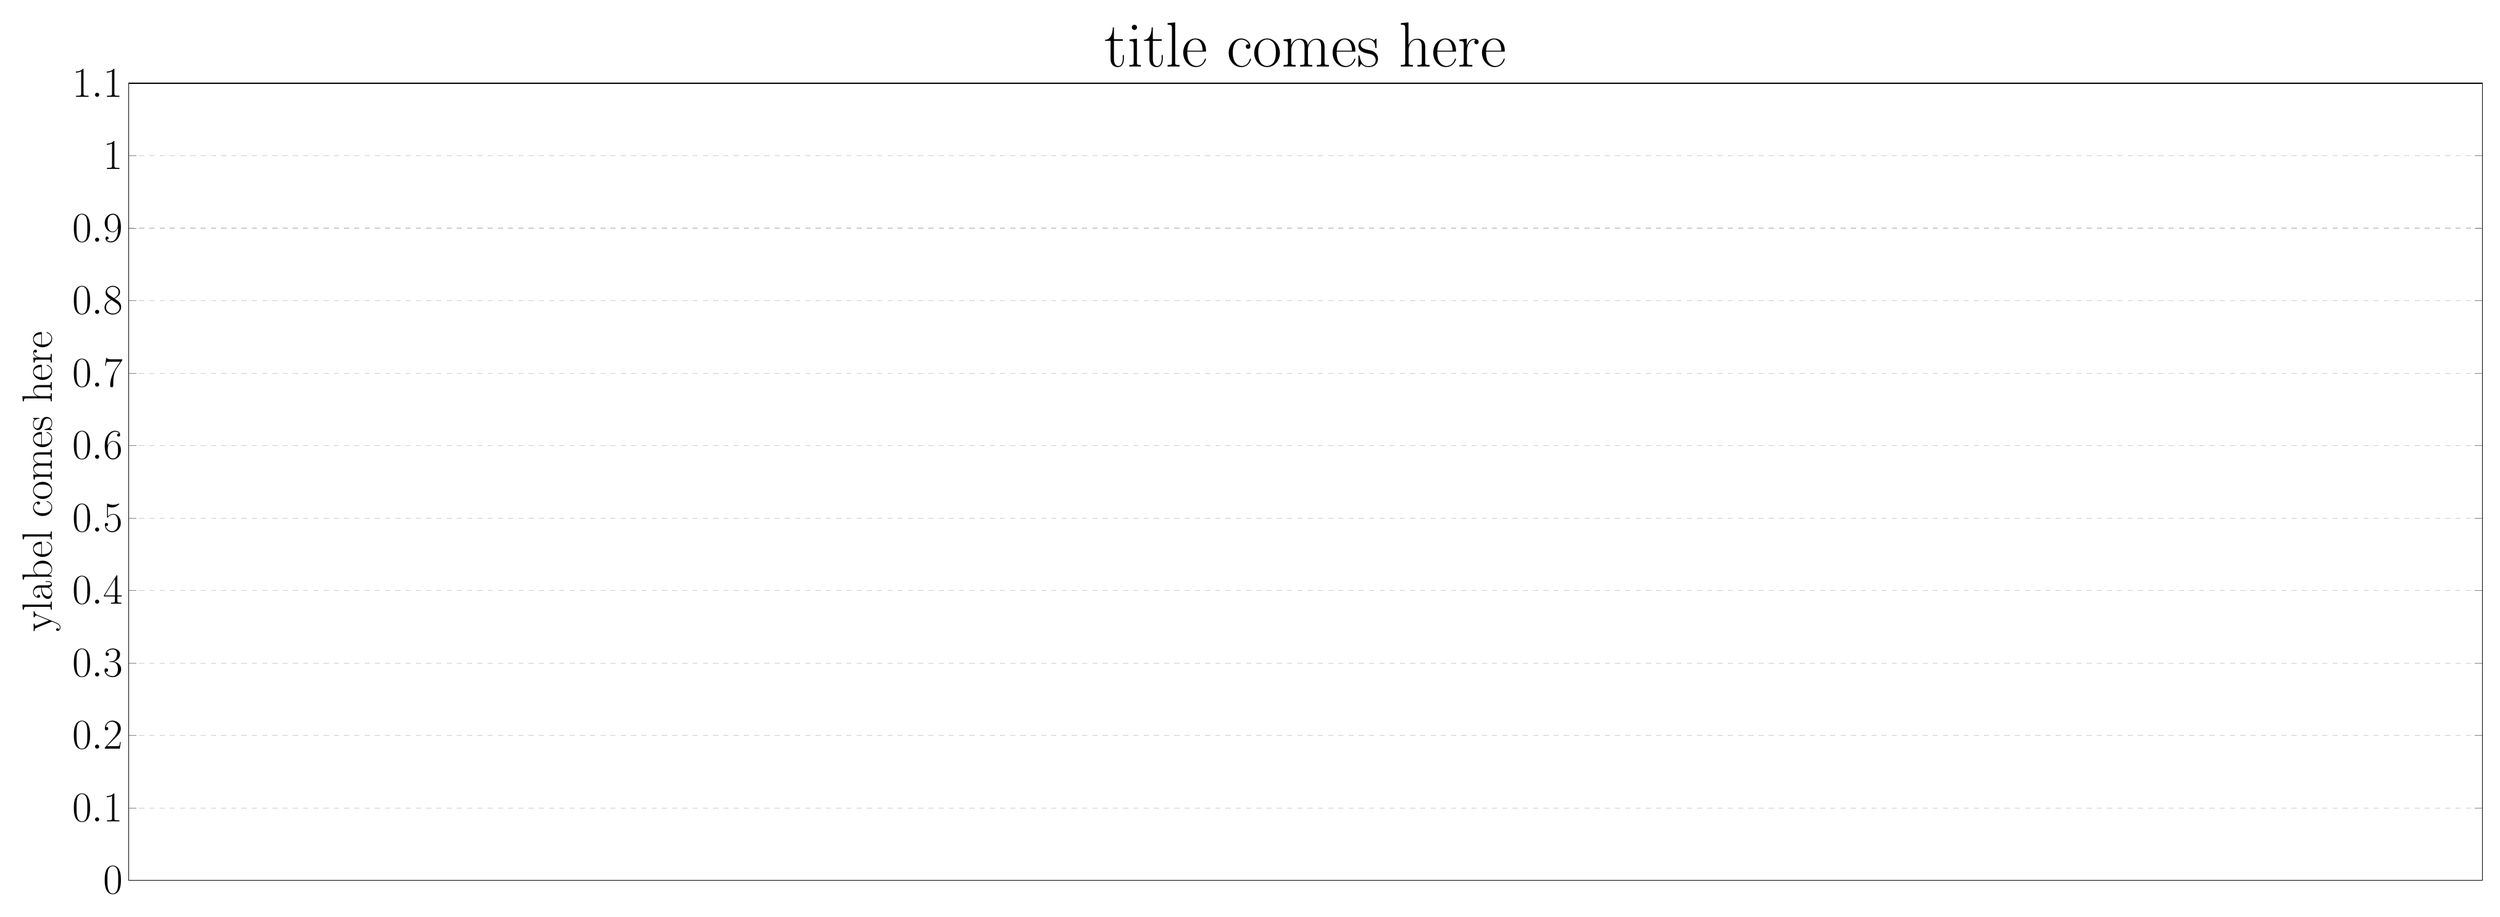
\begin{tikzpicture}
		%	\node at (13.25,15) {\LARGE{title comes here}};
			\begin{axis}[
		%	xmin=0.25, xmax=7.25,
			ymin=0, %ymax=3.25,
			xtick= ,
		%	ytick={0,0.5,1,1.5,2,2.5,3},
			xticklabels= ,
			width  = 50cm,
			height = 18cm,
			major x tick style = transparent,
			%	minor ytick={1, 5, 10, 15, 20, 25, 30 ,35,40},
			grid = minor,	
			%add_bar_commands
			ymajorgrids = true,
			grid style={dashed, gray!40},
			ylabel = {\Huge{ylabel comes here}},
		%	symbolic x coords={Graphene-2048-2048, Graphene-4096-4096, Spin-24-24-24},
			x tick label style={rotate=90, anchor=north east, inner sep=0mm, font={\Huge}},
			tick label style={font={\Huge}},
			scaled y ticks = false,
			enlarge x limits=0.035,
			legend cell align=left,
			legend style={font=\Huge},
			legend columns=-1,
			legend style={
				%at={(1,1.05)},
				%anchor=south east,
				%column sep=1ex,
				legend pos=north east
			},
			%spl_legend_code
			title= {\Huge\scalebox{1.5}{{title comes here}}}
			]

	%addplot cmd

	\legend{legend comes here}

	\end{axis}			
\end{tikzpicture}

\end{document}

